%%
%% This is file `sample-sigchi-a.tex',
%% generated with the docstrip utility.
%%
%% The original source files were:
%%
%% samples.dtx  (with options: `sigchi-a')
%% 
%% IMPORTANT NOTICE:
%% 
%% For the copyright see the source file.
%% 
%% Any modified versions of this file must be renamed
%% with new filenames distinct from sample-sigchi-a.tex.
%% 
%% For distribution of the original source see the terms
%% for copying and modification in the file samples.dtx.
%% 
%% This generated file may be distributed as long as the
%% original source files, as listed above, are part of the
%% same distribution. (The sources need not necessarily be
%% in the same archive or directory.)
%%
%% The first command in your LaTeX source must be the \documentclass command.
\documentclass[sigchi-a,screen]{acmart}

\usepackage[footnotes,definitionLists,hashEnumerators,smartEllipses,hybrid]{markdown}

%%
%% \BibTeX command to typeset BibTeX logo in the docs
\AtBeginDocument{%
  \providecommand\BibTeX{{%
    \normalfont B\kern-0.5em{\scshape i\kern-0.25em b}\kern-0.8em\TeX}}}

%% Rights management information.  This information is sent to you
%% when you complete the rights form.  These commands have SAMPLE
%% values in them; it is your responsibility as an author to replace
%% the commands and values with those provided to you when you
%% complete the rights form.
\copyrightyear{2019}
\acmYear{2019}
\setcopyright{rightsretained}

%% These commands are for a PROCEEDINGS abstract or paper.
\acmConference{CSCW 2019 Workshop - Mapping the "How" of Collaborative Action}{November 10, 2019, Austin TX, USA}
% \acmDOI{no DOI}
% \acmISBN{no ISBN}
% \acmBooktitle{No Booktitle}


%%
%% Submission ID.
%% Use this when submitting an article to a sponsored event. You'll
%% receive a unique submission ID from the organizers
%% of the event, and this ID should be used as the parameter to this command.
%%\acmSubmissionID{123-A56-BU3}

%%
%% The majority of ACM publications use numbered citations and
%% references.  The command \citestyle{authoryear} switches to the
%% "author year" style.
%%
%% If you are preparing content for an event
%% sponsored by ACM SIGGRAPH, you must use the "author year" style of
%% citations and references.
%% Uncommenting
%% the next command will enable that style.
%%\citestyle{acmauthoryear}

%%
%% end of the preamble, start of the body of the document source.
\begin{document}

%%
%% The "title" command has an optional parameter,
%% allowing the author to define a "short title" to be used in page headers.
\title[Processes in Software Citation]{Studying Processes in Software Citation Towards Improved Collaboration Among Scientists}

%%
%% The "author" command and its associated commands are used to define
%% the authors and their affiliations.
%% Of note is the shared affiliation of the first two authors, and the
%% "authornote" and "authornotemark" commands
%% used to denote shared contribution to the research.
\author{Cai Fan Du}
\email{cfdu@utexas.edu}
\orcid{????}
\author{Johanna Cohoon}
\email{jlcohoon@utexas.edu}
\orcid{0000-0002-3352-9766}
\author{James Howison}
% \authornotemark[1]
\email{jhowison@ischool.utexas.edu}
\orcid{0000-0002-5702-149X}
\affiliation{%
  \institution{The University of Texas at Austin}
  \streetaddress{1616 Guadalupe Street}
  \city{Austin}
  \state{TX}
  \postcode{78701-1213}
}

\author{Jason Priem}
\email{jason@ourresearch.org}
\orcid{????}
\author{Heather Piwowar}
\email{heather@ourresearch.org}
\orcid{????}
\affiliation{
  \institution{Our Research Inc.}
  \city{Vancouver}
  \state{BC, Canada}
}

% \author{Lars Th{\o}rv{\"a}ld}
% \affiliation{%
%   \institution{The Th{\o}rv{\"a}ld Group}
%   \streetaddress{1 Th{\o}rv{\"a}ld Circle}
%   \city{Hekla}
%   \country{Iceland}}
% \email{larst@affiliation.org}


%% By default, the full list of authors will be used in the page
%% headers. Often, this list is too long, and will overlap
%% other information printed in the page headers. This command allows
%% the author to define a more concise list
%% of authors' names for this purpose.
\renewcommand{\shortauthors}{Du, Cohoon, and Howison}

%%
%% The abstract is a short summary of the work to be presented in the
%% article.
\begin{abstract}
   We are trying to understand the process of when and how the use of scientific software generates reputational reward for scientific software contributors. At a more micro level, we are studying the processes surrounding software citation by researchers, tool producers, and publishers.  Simultaneously, we are also building a tool, called CiteAs, designed to improve the implementation and usefulness of software citation. Ultimately, we are interested in increasing collaboration in scientific software work. Our method is two-fold: we are conducting artifact-supported interviews and building a publicly available tool.
\end{abstract}

%%
%% The code below is generated by the tool at http://dl.acm.org/ccs.cfm.
%% Please copy and paste the code instead of the example below.
%%
\begin{CCSXML}
<ccs2012>
<concept>
<concept_id>10003120.10003130.10011762</concept_id>
<concept_desc>Human-centered computing~Empirical studies in collaborative and social computing</concept_desc>
<concept_significance>500</concept_significance>
</concept>
</ccs2012>
\end{CCSXML}

\ccsdesc[500]{Human-centered computing~Empirical studies in collaborative and social computing}

%%
%% Keywords. The author(s) should pick words that accurately describe
%% the work being presented. Separate the keywords with commas.
\keywords{process, practice studies, empirical methods, scientific software, software citation}


%%
%% This command processes the author and affiliation and title
%% information and builds the first part of the formatted document.
\maketitle

\section{Why are the processes in software citation of interest}

Software has been increasingly critical in scientific research. However, scientific software work has yet to fully find its place in research practice. Scientific work is dominated by a reputation economy based on the currency of scientific publications and citations~\cite{howison2011scientific}. Scientific software work is often seen as "service work", staying largely invisible inside the system of citation and publication.

Earlier empirical work~\cite{howison2013incentives,howison2011scientific} reveals that contributors to scientific software believed that due credit was not given and that the use value of the software may not justify their time and effort spent on the building of software. 

One way of more fully integrating software work into the scientific reward system is by encouraging users to cite software in their publications. In this way, contributors to the scientific software work might demonstrate their impact and receive reputational reward~\cite{howison2015understanding}.

In reality, the implementation of software citation is hard. Though scientific policy-makers, advocacy groups, and some publishers have been intervening to put software citation into action, there still exist challenges. Park and Wolfram ~\cite{park2019research}, for example, showed that formal software citation practices are still relatively uncommon and that persistent identifiers like DOIs do not necessarily improve citation rates. Katz et al~\cite{katz2019software}, have enumerated a set of existing technical and stakeholder challenges in implementing software citation.

To implement software citation is to introduce behavioral change into the daily practice of researchers and other stakeholders. Therefore, we need to understand the existing practices surrounding software citation in order to identify entry points for effective intervention.

\section{Specific practices that we are trying to reconstruct}

We are seeking to understand processes surrounding software citation at two different levels. At the macro level, we are trying to understand when and how the use of a piece of scientific software generates reputational reward for the creators of the software. Such reward is expected to incentivize high-quality software work, especially through the collaboration among scientists. At a more micro level, we investigate the specific processes occurring at three key locations inside the system:

\begin{itemize}
    \item Contributors making software available: how would they prefer to be cited or credited? How do they make this preference clear?
    \item Researchers authoring a paper: How do they come to the decision of what and how to cite. Can they find software authors' citation requests? Do they know how to format a useful software citation?
    \item The paper review and publication process: When and how are citations reviewed? What citation guidelines are available?
\end{itemize}

\section{How are we studying these processes?}

Our approach is two-fold: First, we are conducting artifact-supported interviews for gaining an in-depth understanding of the localized processes; second, we have been developing a system called CiteAs to identify correct software citations~\cite{priem01cite}. In this way, we complement our research with a tool for intervention.

The artifact-supported interviews are designed for reconstructing our focal periods inside the system. The key is to reestablish critical moments from informant narratives, specifically discussing their past actions and underlying reasoning. We have developed an interview protocol tailored to each stakeholder role: end-user researchers, scientific software contributors, and academic publishers and journal reviewers. We seek to keep the interviews concrete by using artifact elicitation techniques. For end-user researchers, we identify their actual research publications and develop our conversation from these publications. For software tool contributors, we ask them to look for software citation requests online and tell us stories of attempts to ask for credit. At the moment, we are still constructing the interview protocol for academic publishers and journal reviewers; we intend to inquire about their actual process of dealing with citations in reviewing and publishing, socially and technologically. Our interview questions also investigate the individual sociotechnical contexts, such as their perception of how other researchers approach software citation, and their use of citation management software, etc.

Our system, CiteAs, has been used as an additional artifact for prompting further contextualized thinking from informants during interviews. Primarily, CiteAs is a specialized search engine deliberately developed for seeking discoverable software citation requests. 

As a specialized search engine, CiteAs takes an input (e.g., name of a software package, URL of a software project page, a DOI, etc.) and looks for requests for citation. The tool follows a set of heuristics seeking a best guess of what the tool authors would like to be cited: Package names are converted to related websites by taking the first result from a search using the name string. Websites are spidered for identifying key phrases (e.g., "citation", "please cite", "citation.html", "citing.html"). Links to github repositories are followed and the repository files searched for specific citation request files (e.g., CITATION, CITATION.ccf, CODEMETA) or linked to language-specific citation files (e.g., R's DESCRIPTION file). DOIs can also be identified and the DOI API will be called to gather citation metadata. The system then returns its best guess of the citation desired by the software contributors, as well as the citation provenance information showing where that guess came from. Besides, we provide a way for users to report poor search results, and urge software contributors to improve the results by making their citation requests more clear and machine-readable.

\section{The challenges of understanding software citation processes}

The overall process of the reputational rewards as incentive feedback for scientific software development is vastly dispersed through time and geography. The systematic effect is substantial, but it arises from many individual actions across many locations at different times. Much of the relevant behaviors are both private and result in omissions from documents (not citing, or not requesting citation). In our interviews, it is clear that many participants haven't actively thought about the topic, following familiar routines and unaware of the ultimate systematic effect. These issues are shared, we imagine, with many attempts to characterize system-level processes and phenomena. 

We understand there exists significant variation in the relevant practices of software citation across scientific fields, but as is often the case with research on sociotechnical systems we don't have a clear sampling frame. Currently, we are snowball sampling our participants and also try to diversify the roles, experience, and disciplinary areas of the participants we are talking to.

\section{Current status of the project}

Thus far we have conducted 5+ hour-long interviews with end-user researchers and 8+ hour-long interviews with scientific software contributors. Their professional roles, academic experience, and scientific fields vary greatly. We are still seeking more interview participants, especially publishers and journal editors to learn about their relevant practices.

Another ongoing endeavor of our project is that we are mannually annotating a dataset of software mentions in publications as the training set for a machine learning module of the system. It is our aim that CiteAs will be able to automatically identify software mentions in research papers and give citation suggestions. Our full conception of CiteAs is illustrated in Figure 1.

\begin{figure}[H]
  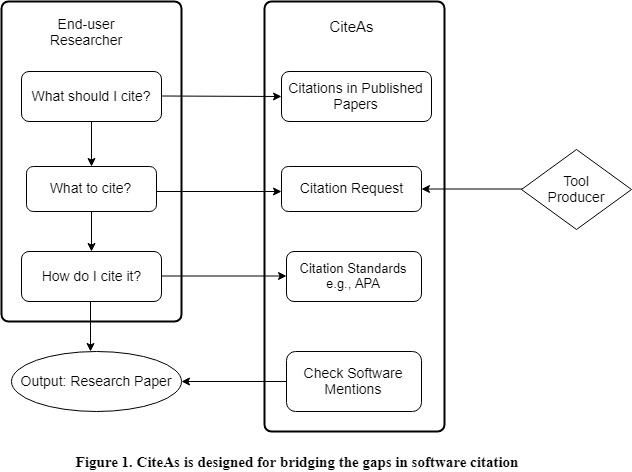
\includegraphics[width=1\textwidth]{SoftciteProcessWorkshop_Figure1.jpg}
\end{figure}

% \section{SIGCHI Extended Abstracts}

% The ``\verb|sigchi-a|'' template style (available only in \LaTeX\ and
% not in Word) produces a landscape-orientation formatted article, with
% a wide left margin. Three environments are available for use with the
% ``\verb|sigchi-a|'' template style, and produce formatted output in
% the margin:
% \begin{itemize}
% \item {\verb|sidebar|}:  Place formatted text in the margin.
% \item {\verb|marginfigure|}: Place a figure in the margin.
% \item {\verb|margintable|}: Place a table in the margin.
% \end{itemize}

%%
%% The acknowledgments section is defined using the "acks" environment
%% (and NOT an unnumbered section). This ensures the proper
%% identification of the section in the article metadata, and the
%% consistent spelling of the heading.
\begin{acks}
This material is based upon work supported by the Sloan Foundation's Digital Science program.
\end{acks}

%%
%% The next two lines define the bibliography style to be used, and
%% the bibliography file.
\bibliographystyle{ACM-Reference-Format}
\bibliography{softcite-ref}

\appendix

\section{Bibliography sketches}

\subsection{Cai Fan Du}
Fan is a doctoral student at the Information School of the University of Texas at Austin. She is interested in studying the organizing of distributed efforts in the production of digital artifacts through a sociotechnical lens. Before graduate school she studied economics and french.

\subsection{Johanna Cohoon}
Johanna (Hannah) Cohoon is a PhD Candidate at the Information School of the University of Texas at Austin where she studies scientific research practices and cyberinfrastructure. Previously, she worked at the Center for Open Science where she researched reproducibility in Psychology. She is interested in how scientific norms and practices change. Johanna received her bachelors degree in Cognitive Science from the University of Virginia. 

\subsection{James Howison}

James Howison is an Associate Professor at the Information School of the University of Texas at Austin, where he has been since August 2011, following a post-doc at CMU and his 2009 PhD from Syracuse Information School. James has studied open source software development and the development of software in science because both are interesting examples of collaboration, and is particularly interested in understanding how different incentives, such as working for fun or for academic reputation, lead to different structures of collaboration. James is a 2019 PECASE award winner, based on a NSF 2014 CAREER award. Publications include MISQ, Information and Organization, and CSCW. \href{http://james.howison.name}{http://james.howison.name}

\end{document}
\endinput
%%
%% End of file `sample-sigchi-a.tex'.
